% Chapter Template

\chapter{Dataset} % Main chapter title

\label{ch:04} % Change X to a consecutive number; for referencing this chapter elsewhere, use \ref{ChapterX}

%----------------------------------------------------------------------------------------
%	SECTION 1
%----------------------------------------------------------------------------------------

\section{Synthetic Dataset}
To train a deep learning model with supervised learning scheme, a dataset should require two principles, truth-worthy ground-truth and comprehensive scenarios. The depth map captured by Kinect is not satisfied the first requirement since it is usually semi-dense with a number of missing pixels, as shown in Figure \ref{fig:kinect-depth}. Therefore, a more elaborate depth map is required for the training work. In this thesis, a dataset called ``synthetic50" is created for the training works.


\subsection{Resource}
\cite{data1}, \cite{data2}, \cite{data3} and \cite{data4} published a set of point cloud dataset on the internet for computer vision task research. These point clouds are scanned from real objects using high resolution scanners like Cyberware 3030 MS+ and calibrated with post processing. Each objects has been scanned for hundreds of times for an exhaustive completion for the origin objects, which is up to millions points. (\cite{data1}). The dense point clouds makes the normal inference task trivial since the neighbor based method performs good enough for these kind of task. Some of the point cloud even equipped with pre-computed normal map based on more advanced methods. They all provides the accurate ground-truth for the supervised learning method.

In this thesis, 50 point clouds scanned on real objects have been used for training work and 5 point clouds have been used for test work. Figure \ref{fig:dataset-demo} illustrates some of the point clouds. Appendix \ref{AppendixA} gives a full version of dataset models.

\begin{figure}[!h]
	\centering
	\begin{subfigure}[b]{0.23\linewidth}
		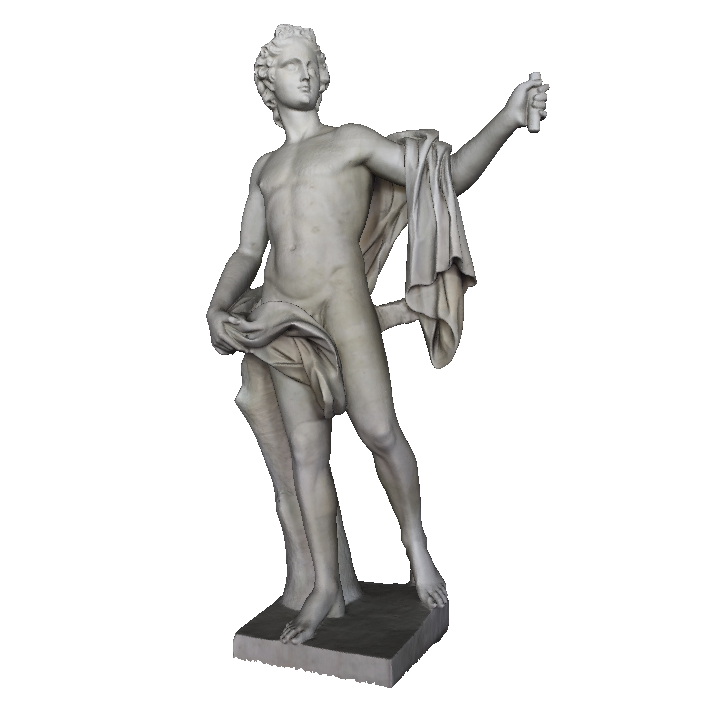
\includegraphics[width=\linewidth]{./Figures/train-dataset/00.apoll.png}
		\caption{apoll}
	\end{subfigure}
	\begin{subfigure}[b]{0.23\linewidth}
		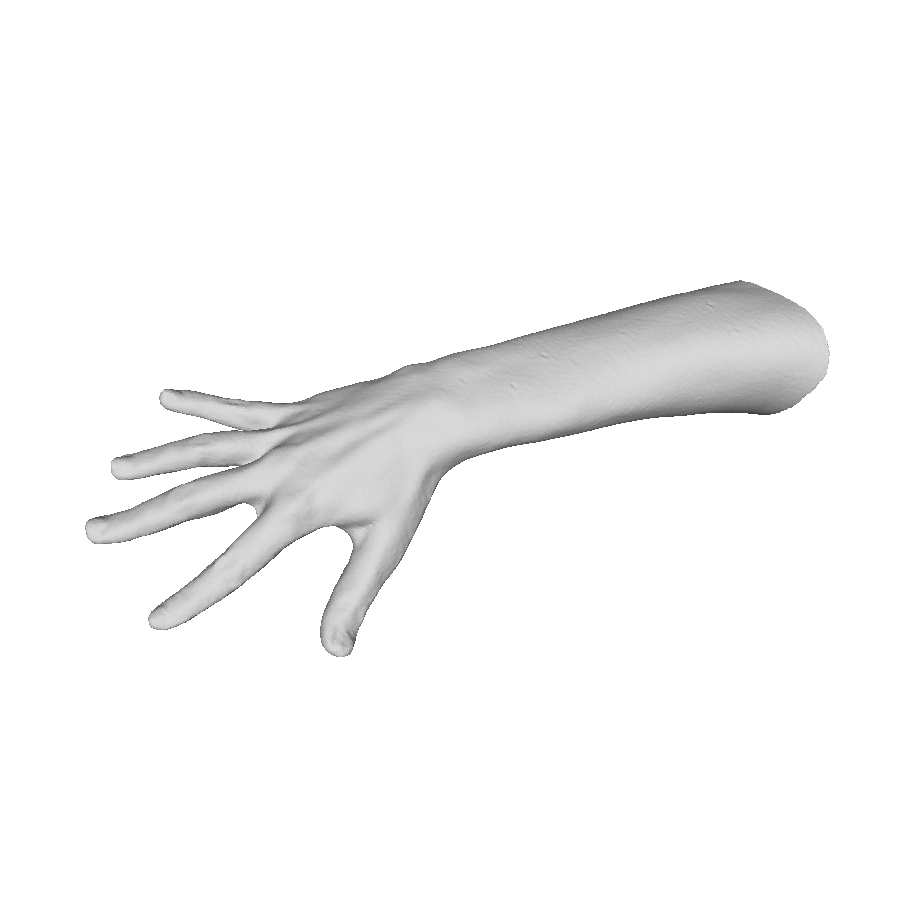
\includegraphics[width=\linewidth]{./Figures/train-dataset/01.arm.png}
		\caption{arm}
	\end{subfigure}
	\begin{subfigure}[b]{0.23\linewidth}
		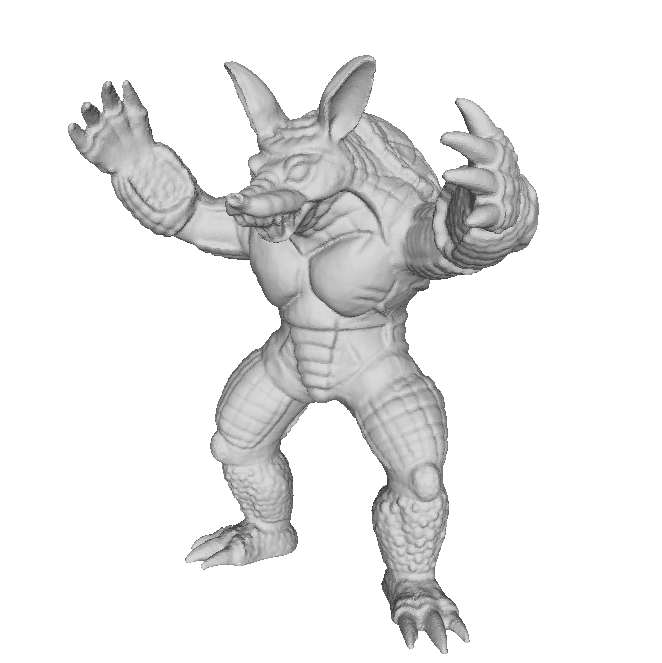
\includegraphics[width=\linewidth]{./Figures/train-dataset/02.armadillo.png}
		\caption{armadillo}
	\end{subfigure}
	\begin{subfigure}[b]{0.23\linewidth}
		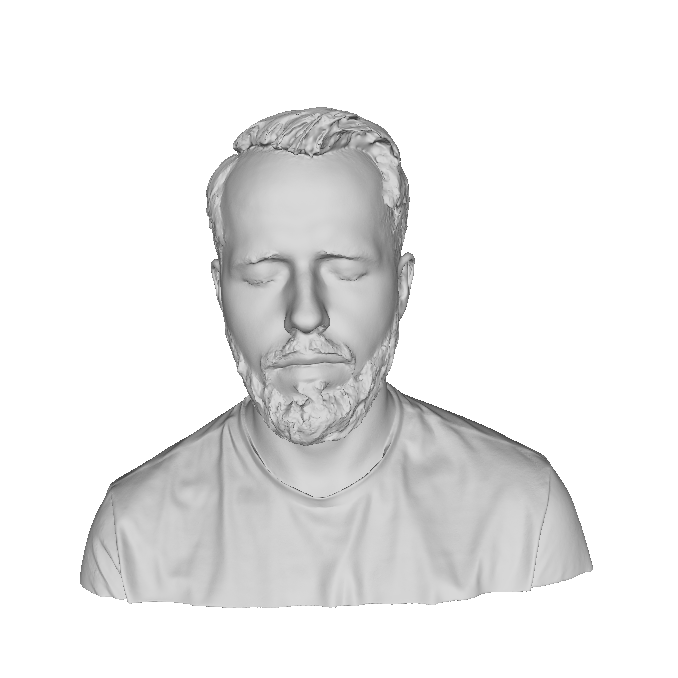
\includegraphics[width=\linewidth]{./Figures/train-dataset/03.bearded-guy.png}
		\caption{bearded-guy}
	\end{subfigure}
	
	\begin{subfigure}[b]{0.23\linewidth}
		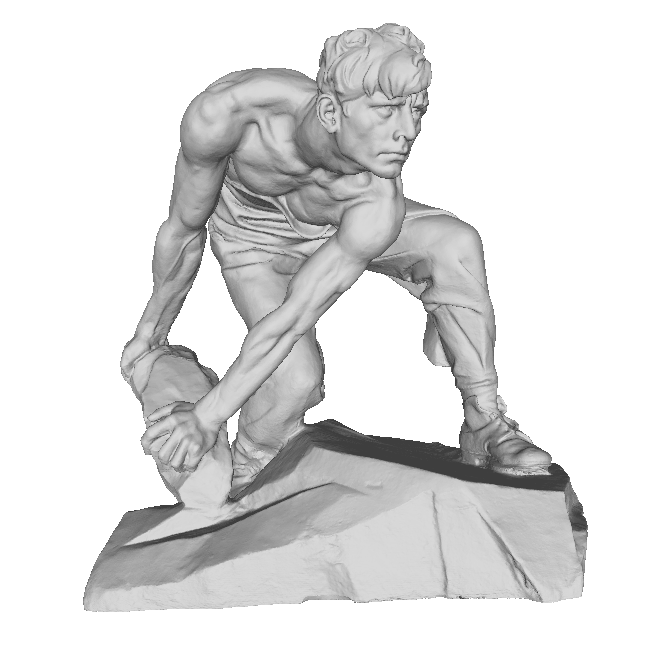
\includegraphics[width=\linewidth]{./Figures/train-dataset/04.bronze-sculpture.png}
		\caption{bronze-sculpture}
	\end{subfigure}
	\begin{subfigure}[b]{0.23\linewidth}
		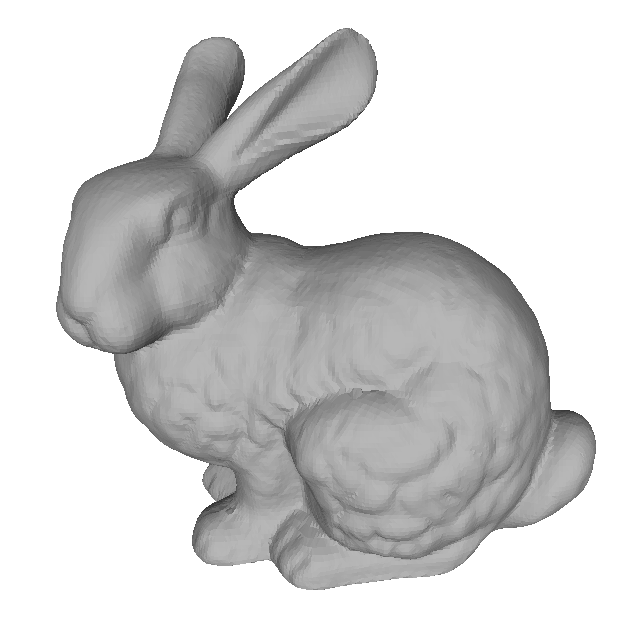
\includegraphics[width=\linewidth]{./Figures/train-dataset/05.bunny.png}
		\caption{bunny}
	\end{subfigure}
	\begin{subfigure}[b]{0.23\linewidth}
		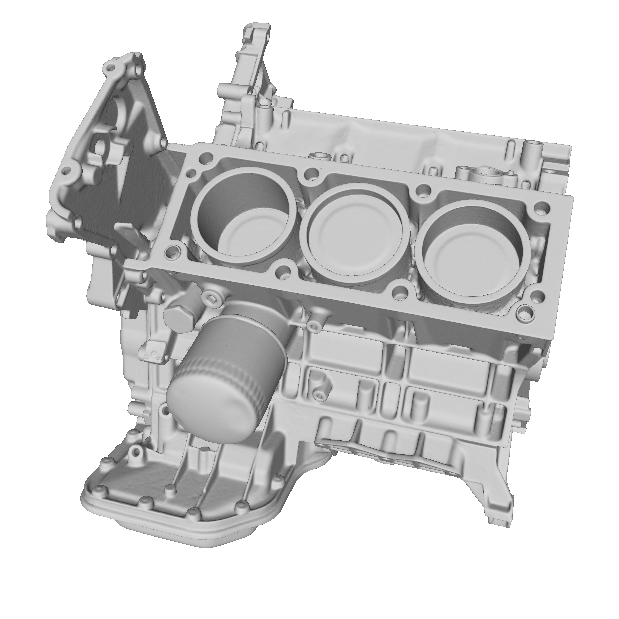
\includegraphics[width=\linewidth]{./Figures/train-dataset/06.car-engine.png}
		\caption{car-engine}
	\end{subfigure}
	\begin{subfigure}[b]{0.23\linewidth}
		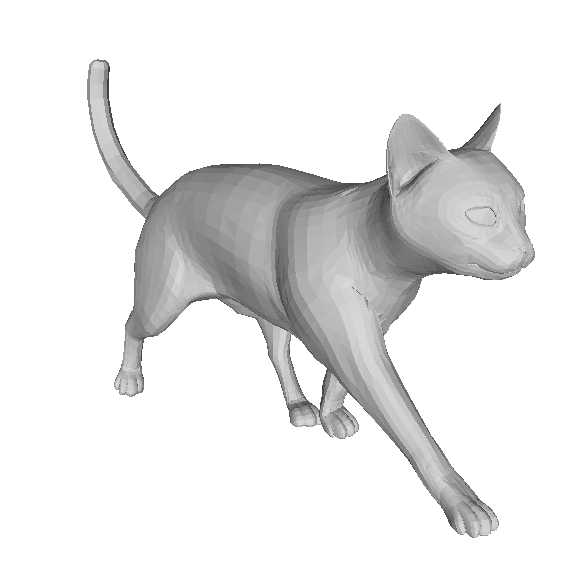
\includegraphics[width=\linewidth]{./Figures/train-dataset/07.cat.png}
		\caption{cat}
	\end{subfigure}
	
	\label{fig:dataset-demo}
	\caption{Point clouds scanned by high resolution scanners}
\end{figure}


\subsection{Data Files}
In order to fit the using scenario of Kinect as much as possible, a set of synthetic 3D scenes of each object is captured via Unity, which is a game engine using for 3D games creation. It can place the point cloud in a virtual   The main advantage using generated scene is the complete information of all the information in the synthetic world. The depth map can be captured in a loss-free way. The corresponding normal map can also be safely considered as ground truth. To construct the dataset, 1000 different scenes have been saved. The model pose, camera position, light position are random changed in each scene.
For each scene, following information is recorded
\begin{itemize}
	\item Depth range
	\item Light position
	\item Camera intrinsic and extrinsic matrix
	\item Depth map
	\item Grayscale image
	\item Normal Map	
\end{itemize}



\begin{itemize}
	\item Grayscale Image
\end{itemize}

In Unity, the grayscale image in acquired via RGB texture by the following equation:
\[ gray: \frac{r+2g+b}{4}  \]



%% What is surface normal
\label{sec:surface-normal}
In three dimension geometry, a surface normal at the point $ P $ is a vector $ n $ perpendicular to the tangent plane of the surface at point $ P $. The length of a normal is usually one, with a sign to represent the sides (interior or exterior).%% add a picture to illustrate


\subsection{Point Cloud}
\label{sec:depth-map-to-point-cloud}

A depth map $ D $ is captured by a depth camera like Kinect, which is a 1 channel image that contains the information relating to the distance of the surfaces of the scene objects from a viewpoint. The range of distance depends on the performance of depth camera. It can be saved as a 16-bit image, i.e. each pixel in range $0 \tilde 65535$. A depth map with knowing calibration can be further converted to a structured point cloud. 


\subsection{Point Cloud calculation}

Consider a 3-dimensional Euclidean space. Use $ z $ axis denotes the depth. The $ x  $ and $ y $ axes perpendicular with each other. For a pixel $ (u,v) $ on depth map, its value $ D(u,v) $ is the $ Z $ component of the 3D point $P_C = (X,Y,Z) $ corresponding the camera origin. Based on the triangle similarity, we can get other two components $ X $ and $ Y $ as follows

\begin{dgroup*}
	
	\begin{dmath*}
		X = \frac{uZ}{fk_u}
	\end{dmath*}
	\begin{dmath*}
		Y = \frac{vZ}{fk_v}
	\end{dmath*}
\end{dgroup*}

where $ fk_u, fk_v $ is the focal length in pixels align $ u $ and $ v $ axes.
It can be further converted to world coordinate system based on extrinsic matrix $ R $ and $ t $, that is
\[P_W = P_CR+t \]

\subsection{Point Cloud Normalization}


\label{sec:dataset-normalization}
%% How to represent input tensor, to make it fast converse

The vertices have been normalized before feed them into the model. The depth range of each scene is shown in Figure \ref{fig:data-range}.
The sizes of each training object are various, whereas it should be as an invariant value for the training model. Thus the normalization is required before feed training objects into the models. Figure \ref{fig:data-range} shows the fluctuation of extreme values and their ranges in 100 random training items. Table \ref{tab:data-range} gives the corresponding average values.
%\begin{figure}[!h]
%	\centering
%	{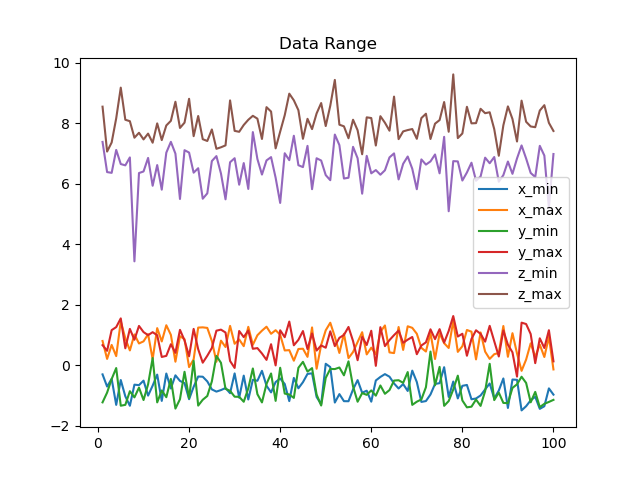
\includegraphics[width=0.45\textwidth]{./pic/Data_Extreme.png}}
%	{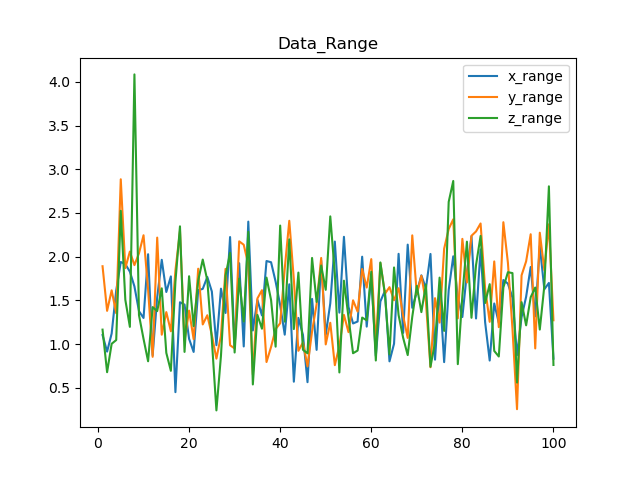
\includegraphics[width=0.45\textwidth]{./pic/Data_Range.png}}
%	\label{fig:data_range}
%	\caption{Left: Extreme value in 3 axis; Right: Vertex range in 3 axis}
%\end{figure}

\begin{table}[!h]
	\centering
	\begin{tabular}{|c|c|c|c|}
		\hline
		Axis & Range & Min & Max\\
		\hline
		X & 1.48 & -0.75 & 0.73\\
		Y & 1.56 & -0.76 & 0.80\\
		Z & 1.47 & 6.53 & 8.00\\
		\hline
	\end{tabular}
	\caption{The ranges and extreme values of each axis. The extreme min and max values of both X axis and Y axis are close to $ -0.75 $ and $ 0.75 $ separately. The case for Z axis is $ 6.5 $ and $ 8.0 $ separately. However, the range of three axes are relatively similar, around 1.5. 
	}
	\label{tab:data-range}
\end{table}


For the normalization, first we translate the point to the original point as much as possible, then choose the range value of one axis as a scale factor, normalize it to a unit object. 

\begin{equation}\label{eq:normalization}
	U^a = (V^a - V^a_{min}) / s  \quad  \text{for } a \text{ in }  X,Y,Z \text{ axis}
\end{equation}
where $ V^a_{min} $ denote the minimum value appeared in axis $ a $, $ s $ is the range of an axis, which can be any one of X, Y, or Z axis. 

In this thesis, the range of X is chosen as scale factor for each scene.



As discussed in \ref{sec:dataset-normalization}, the 3D vertex point cloud should be moved to origin point and normalize in range $ [0,1] $ to acquire a scale invariant feature.


\begin{dgroup*}
	
	\begin{dmath*}
		X_n =\frac{X-\min(X)}{s}
	\end{dmath*}
	\begin{dmath*}
		Y_n = \frac{Y-\min(Y)}{s}
	\end{dmath*}
	
	\begin{dmath*}
		Z_n = \frac{Z-\min(Z)}{s}
	\end{dmath*}
	
	
\end{dgroup*}

where $ s $ is a scale factor, 

\begin{dmath*}
	s = \max(X)-\min(X)
\end{dmath*}
It is calculated as the range in $ X $ axis, but theoretically can be used by $ Y $ or $ Z $ axes as well.




\subsection{Noise}
\label{sec:noise}
The raw depth maps captured by Kinect usually have missing pixels. As shown in Figure \ref{fig:depth_map_kinect}.
Observing the depth map, the missing pixels distributed all around the scene. Therefore an uniformly distributed pixel-delete noise is used for noise simulation. 
It is reasonable that the noise intensities in different scenes are various. Some scenes have more missing pixels and some have less. It enables the model to not only learn scenarios with noise, but also with small minority noise or even without noise. In the noised dataset, the noise intensity is a x-percent pixel dropoff operation. For example, noise-intensity-10 means removes 10\% pixels.
Figure \ref{fig:noise-intensity} shows the visualization of depth map after adding noise.
%% add noise image
\begin{figure}[!h]
	\centering
	{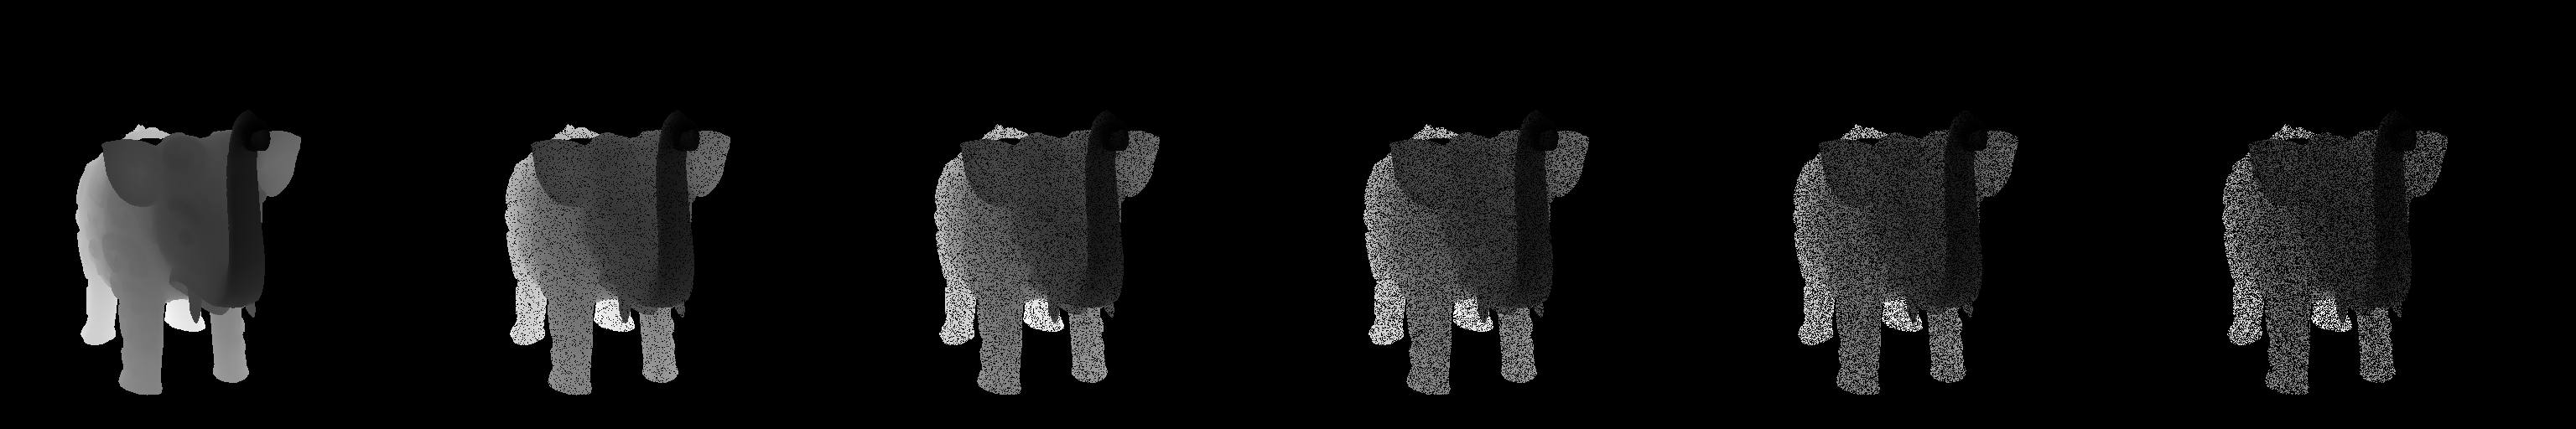
\includegraphics[width=.9\textwidth]{./Figures/add_noise_depth.png}}
	\decoRule	
	\caption{Noise-intensity on 0, 10, 20, 30, 40, 50. Object Name: elephant-zun-lid.}
	\label{fig:noise-intensity}
\end{figure}


\subsection{Fit to PyTorch}
In order to saving the training time, the dataset is compressed in PyTorch format. The structure of a single item is shown in Table \ref{tab:tensor-structure}.
\begin{table}
	\caption{The structure of a single tensor in the dataset.}
	\label{tab:tensor-structure}
	\centering
	\begin{tabular}{l l}
		\toprule
		\tabhead{Name} & \tabhead{Description} \\
		\midrule
		\multirow{3}{*}{input-tensor}  & Vertex \\  & Image \\  & Light Direction \\
		\hline
		\multirow{4}{*}{output-tensor}  & GT-Normal  \\ & GT-Normal * GT-Light-Direction \\ & Image \\ & GT-Light-Direction \\
		\hline
		Light position & light position \\
		\hline 
		\multirow{3}{*}{Camera Matrix}  & K \\  & R \\  & t \\
		\hline 
		\multirow{2}{*}{Depth Range}  & minDepth \\  & maxDepth \\
		\hline
		\bottomrule\\
	\end{tabular}
\end{table}




\section{Real Dataset}

The real dataset is the depth map and rgb image captured via Kinect...


\section{Metrics for evaluation}
Angle Loss

